\chapter{Experimental Evaluation}
\label{chap5}

At this point, we have described our primary motivation and background, and comprehensively analyzed the architecture and implementation of our application. In this section, we execute a series of realistic routines to demonstrate the key principles of our implementation. We test the data validation process and message size reduction. Finally, we deploy a realistic number of producer clients, generating data for our Kafka cluster, so that we can evaluate its throughput. 
%Finally, we employ AMQP and MQTT clients to determine whether there is a significant delay difference between native Kafka producers and Connect ones.

\section{Data Validation Routine}

In order to test our data validation routine we have prepared a set of scenarios, configuring our schema, Figure \ref{json_avro}, depending on the use cases and our needs.

\begin{enumerate}
    \item Firstly, we can configure all fields in our schema, to default to null values. This allows for normal event parsing to our Kafka Cluster even if any fields in our JSON input file are missing. While this configuration offers maximum flexibility, it does not check our data before it is published to our application.
    \item In the second scenario, we select a few or just one value to default to null. For instance, we could set our temperature field to null in our schema if a group of sensors or devices doesn't support this measurement. In this instance, messages would still be parsed even if the temperature field was missing from the input messages.
    \item The third scenario involves not setting any field to default at null. This enforces strict data validation, requiring all our fields to be included in our input file.
    \item The fourth case involves disallowing additional fields beyond those included in the schema fields. By default, the schema registry permits extra fields if the required ones have been validated. For example, if an incoming message includes an additional 'pressure' field, we can decide whether or not we want this event to be produced.
\end{enumerate}

In the four scenarios outlined, our goal was to showcase the versatility of our schema registry implementation. As a result, we ranged from a highly flexible data validation routine to a very strict one. The degree of flexibility is dependent on the requirements of our application and implementation at each instance. This underscores the importance of maintaining a balance between adaptability of data and its consistency.

\definecolor{color1}{RGB}{133,147,148}
\definecolor{color2}{RGB}{29,52,94}


\section{Event Size Reduction}

\begin{table}[htbp]
\centering
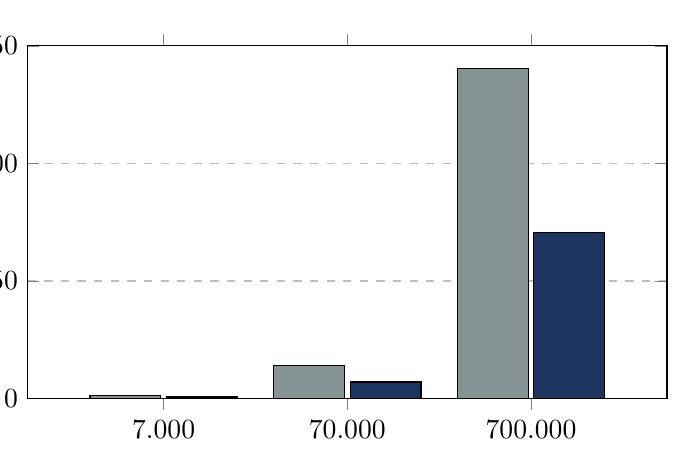
\begin{tikzpicture}[trim axis left, trim axis right]
\begin{axis}[
    ybar,
    bar width=0.9cm,
    width=0.8\textwidth,
    height=0.5\textwidth,
    ylabel={MegaBytes},
    symbolic x coords={7.000, 70.000, 700.000},
    xtick=data,
    ymin=0,
    ymax=150,
    enlarge x limits=0.37,
    ymajorgrids = true,
    grid style={dashed}
    ]
\addplot[fill=color1] coordinates {(7.000, 1.402) (70.000, 14.02) (700.000, 140.19)};
\addplot[fill=color2] coordinates {(7.000, 0.707) (70.000, 7.076) (700.000, 70.76)};
\end{axis}
\end{tikzpicture}
\caption{JSON to Avro size of messages comparison }
\label{avro_vs_json}
\end{table}
Our Schema Registry implementation enables us to store events in our cluster in a more compact and efficient manner. We produced a set of messages to observe the size reduction between native or string JSON format messages, and Avro serialized ones. Our data sets are in groups of 7,000, 70,000, and 700,000. As presented in table \ref{avro_vs_json}, the size reduction ranges from 1,402 KB to 707 KB, 14.02 MB to 7.076 MB, and 140.19 MB to 70.76 MB, for the batched 7,000, 70,000 and 700,000 messages respectively. Therefore, the reduction rate for our input message when converted to Avro format is $\approx$ 48-50\%. This size reduction can vary based on the structure of the original fields and the initial event size, and it can be increased even further. Although the size reduction in our case is in the range of megabytes, it is clear that this sets the stage for larger scale implementations where tens or even hundreds of millions of events are constantly stored in the clusters.



\section{Throughput Testing}

We have created a realistic deployment scenario to test whether our implementation can handle the expected payload. In this scenario, we emulate a situation with a hundred devices producing data, setting up a hundred producers that constantly send data to our Kafka cluster. However, in our tests, we produce messages every second and every five minutes. This dual frequency approach provides a clear view of the volume of messages our implementation can handle, both with our standard deployment frequency, and with a significantly higher one.
Often, benchmarks test throughput in unrealistic environments. By conducting realistic tests, we can confirm that our implementation can handle the load during production. We leverage Kafka's partition mechanism in this process, with each of the hundred devices representing a hundred partitions. This is an optimal use case where each partition is connected to a single device.

Given that our production message frequency is every five minutes, by sending messages every second in our cluster, we emulate the behaviour of having a significantly larger number of devices publishing messages. It is also important to note that throughput results often depend on the event message size. 
Therefore, we conduct our experiment using our application's message structure. The experimentation was carried out on an i7-6700k system, utilizing Docker engine hosted on WSL2, with an allocation of 6 logical cores. Our implementation was able to handle incoming messages at frequencies of both every second and every five minutes without any downtime. Similarly, our consumer was able to read data without any downtime, even during the test with a frequency of every second. As a result, we have verified that our cluster implementation can handle a hundred messages being sent every second from a hundred different devices, based on our given system configuration.